\documentclass[12pt,a4paper]{article}

% Język polski i kodowanie
\usepackage[polish]{babel}
\usepackage[T1]{fontenc}
\usepackage[utf8]{inputenc}

% Pakiety graficzne i tabel
\usepackage{graphicx}
\usepackage{float}
\usepackage{booktabs}
\usepackage{tabularx}
\usepackage{geometry}
\usepackage{fancyhdr}
\usepackage{titlesec}
\usepackage{caption}
\usepackage{subcaption}

% Konfiguracja marginesów
\geometry{margin=2.5cm}

% Interaktywny spis treści z usuniętymi obwódkami linków
\usepackage{hyperref}
\hypersetup{
    colorlinks=true,
    linkcolor=black,
    filecolor=black,
    urlcolor=blue,
    citecolor=black,
    pdfborder={0 0 0}
}

% Ustawienia nagłówka i stopki
\setlength{\headheight}{15pt}
\pagestyle{fancy}
\fancyhf{}
\fancyhead[L]{StegoCloud -- Dokumentacja Projektu}
\fancyhead[R]{\thepage}
\fancyfoot[C]{Politechnika Łódzka -- ZZPJ 2026}
\renewcommand{\headrulewidth}{0.4pt}
\renewcommand{\footrulewidth}{0.4pt}

% Ustawienia formatowania listingów
\usepackage{listings}
\usepackage{xcolor}
\lstset{
    basicstyle=\ttfamily\small,
    backgroundcolor=\color{gray!10},
    frame=single,
    breaklines=true,
    captionpos=b
}

\begin{document}

% --- STRONA TYTUŁOWA ---
\begin{titlepage}
    \centering
    \vspace*{1cm}
    {\large\bfseries Politechnika Łódzka} \\
    \vspace*{0.2cm}
    {\large Wydział Fizyki Technicznej, Informatyki i Matematyki Stosowanej} \\
    \vspace*{0.2cm}
    {\large Instytut Informatyki} \\
    \vspace*{2cm}
    
    \vspace*{1.5cm}
    
    {\Huge\bfseries StegoCloud} \\
    \vspace*{0.5cm}
    {\Large\bfseries System mikroserwisowy do ukrywania i odczytywania szyfrowanych znaków wodnych w obrazach PNG} \\
    \vspace*{1cm}
    {\large Dokumentacja techniczna i projektowa} \\
    \vspace*{0.5cm}
    {\large Przedmiot: Zaawansowane Zagadnienia Programowania w Javie} \\
    \vspace*{2cm}
    
    \begin{flushleft}
        \large
        \textbf{Członkowie zespołu projektowego:} \\
        \vspace*{0.2cm}
        \begin{tabular}{ll}
            Bartosz Kołaciński & index: 251554 \\
            Mateusz Kosowski & index: 251558 \\
            Nikodem Nowak & index: 251598 \\
            Wiktor Pankanin & index: 251606 \\
            Jakub Rosiak & index: 251620 \\
            Jakub Rusek & index: 247774 \\
        \end{tabular}
    \end{flushleft}
    
    \vfill
    {\large Łódź, Czerwiec 2026}
\end{titlepage}

\newpage

% --- SPIS TREŚCI ---
{
  \hypersetup{linkcolor=black}
  \tableofcontents
}
\newpage

% --- 1. WPROWADZENIE ---
\section{Wprowadzenie}

\subsection{Cel projektu}
Głównym celem projektu \textbf{StegoCloud} jest zaprojektowanie oraz implementacja nowoczesnego, rozproszonego i bezpiecznego systemu do dystrybucji i weryfikacji obrazów cyfrowych za pomocą ukrytych (niewidocznych) znaków wodnych. System pozwala autorom oraz dystrybutorom treści multimedialnych (np. obrazów PNG) na weryfikację ich oryginalności oraz identyfikację ewentualnego źródła przecieku lub nieautoryzowanego użycia, przy jednoczesnym zabezpieczeniu samej treści znaku wodnego przed odczytem przez osoby nieuprawnione.

\subsection{Zakres projektu}
System został zaprojektowany w nowoczesnej architekturze mikroserwisowej i obejmuje:
\begin{itemize}
    \item \textbf{Usługi autoryzacji i rejestracji} zarządzające tożsamościami użytkowników i ról (Zwykły Użytkownik, Administrator).
    \item \textbf{Moduł subskrypcyjny} realizujący logikę biznesową planów taryfowych (\texttt{FREE}, \texttt{STANDARD}, \texttt{PRO}) oraz dynamiczne zarządzanie saldem i rezerwacjami tokenów użytkowników.
    \item \textbf{Serwis znakowania (watermarkingu)} oparty o zaawansowany silnik w języku Python osadzający zaszyfrowane komunikaty w dziedzinie częstotliwościowej (DCT) obrazów PNG.
    \item \textbf{Serwis sztucznej inteligencji (AI)} dokonujący klasyfikacji zawartości obrazów przy użyciu modelu \texttt{MobileNetV2} w środowisku uruchomieniowym ONNX.
    \item \textbf{Interfejs graficzny użytkownika (GUI)} zrealizowany w technologii Svelte, pozwalający na łatwe korzystanie z funkcji platformy.
\end{itemize}

\subsection{Grupa docelowa (Do kogo projekt jest skierowany)}
StegoCloud jest skierowany przede wszystkim do:
\begin{itemize}
    \item \textbf{Twórców cyfrowych i fotografów} chcących trwale zabezpieczyć swoje prace przed kradzieżą i niekontrolowanym rozpowszechnianiem.
    \item \textbf{Agencji reklamowych i marketingowych} dystrybuujących materiały graficzne do klientów zewnętrznych, które muszą pozostać poufne do momentu oficjalnej publikacji.
    \item \textbf{Systemów zarządzania treścią (CMS) i platform e-commerce} w celu automatycznego stemplowania pobieranych obrazów tożsamością kupującego (śledzenie nielegalnej redystrybucji).
\end{itemize}

\newpage

% --- 2. OPIS SYSTEMU ---
\section{Opis systemu}

\subsection{Przeznaczenie}
Platforma StegoCloud służy do bezpowrotnego, niewidocznego dla ludzkiego oka stemplowania cyfrowych plików PNG. W przeciwieństwie do widocznych znaków wodnych, które można łatwo wyciąć lub zamazać, steganografia w dziedzinie częstotliwościowej (Discrete Cosine Transform -- DCT) osadza informacje bezpośrednio w strukturze pikseli obrazu. Znak wodny chroniony jest kryptograficznie (AES-GCM) oraz nadmiarowo (Reed-Solomon Error Correction Code), co zapobiega fałszowaniu i pozwala na poprawny odczyt nawet przy drobnych zniekształceniach.

\subsection{Główne funkcje}
System oferuje następujące operacje taryfikowane odpowiednim kosztem tokenowym:
\begin{enumerate}
    \item \textbf{Capacity Check (0 tokenów)}: Analizuje obraz PNG i informuje o maksymalnej liczbie bajtów, jakie można w nim ukryć w zależności od jego wymiarów (minimalny rozmiar to $1024 \times 1024$ pikseli).
    \item \textbf{Embed (5 lub 8 tokenów)}: Osadza zaszyfrowany i zabezpieczony kodem korekcyjnym tekst w obrazie. Rozmiary poniżej Full HD ($1920 \times 1080$) zużywają 5 tokenów (tier \texttt{EMBED\_768}), większe 8 tokenów (tier \texttt{EMBED\_1024}).
    \item \textbf{Detect (1 token)}: Sprawdza, czy w przesłanym obrazie znajduje się poprawny znak wodny i określa jego właściciela.
    \item \textbf{Extract (2 tokeny)}: Wyodrębnia ukryty tekst. Zwykły użytkownik może odczytać tylko swoje znaki wodne, administrator ma uprawnienia do wszystkich.
    \item \textbf{Visualize (3 tokeny)}: Generuje mapę ciepła (heatmap) pokazującą bezwzględne różnice wartości pikseli przed i po osadzeniu znaku wodnego.
    \item \textbf{AI Classification (2 tokeny)}: Opcjonalna klasyfikacja zawartości obrazu przy pomocy modelu sieci neuronowej MobileNetV2 (dostępna tylko dla planu \texttt{PRO}).
\end{enumerate}

\subsection{Architektura systemu}
Projekt zrealizowano w architekturze mikroserwisowej z wykorzystaniem stosu technologicznego Spring Cloud oraz kontenerów Docker. Diagram przedstawia strukturę powiązań pomiędzy komponentami systemu.

\begin{figure}[H]
    \centering
    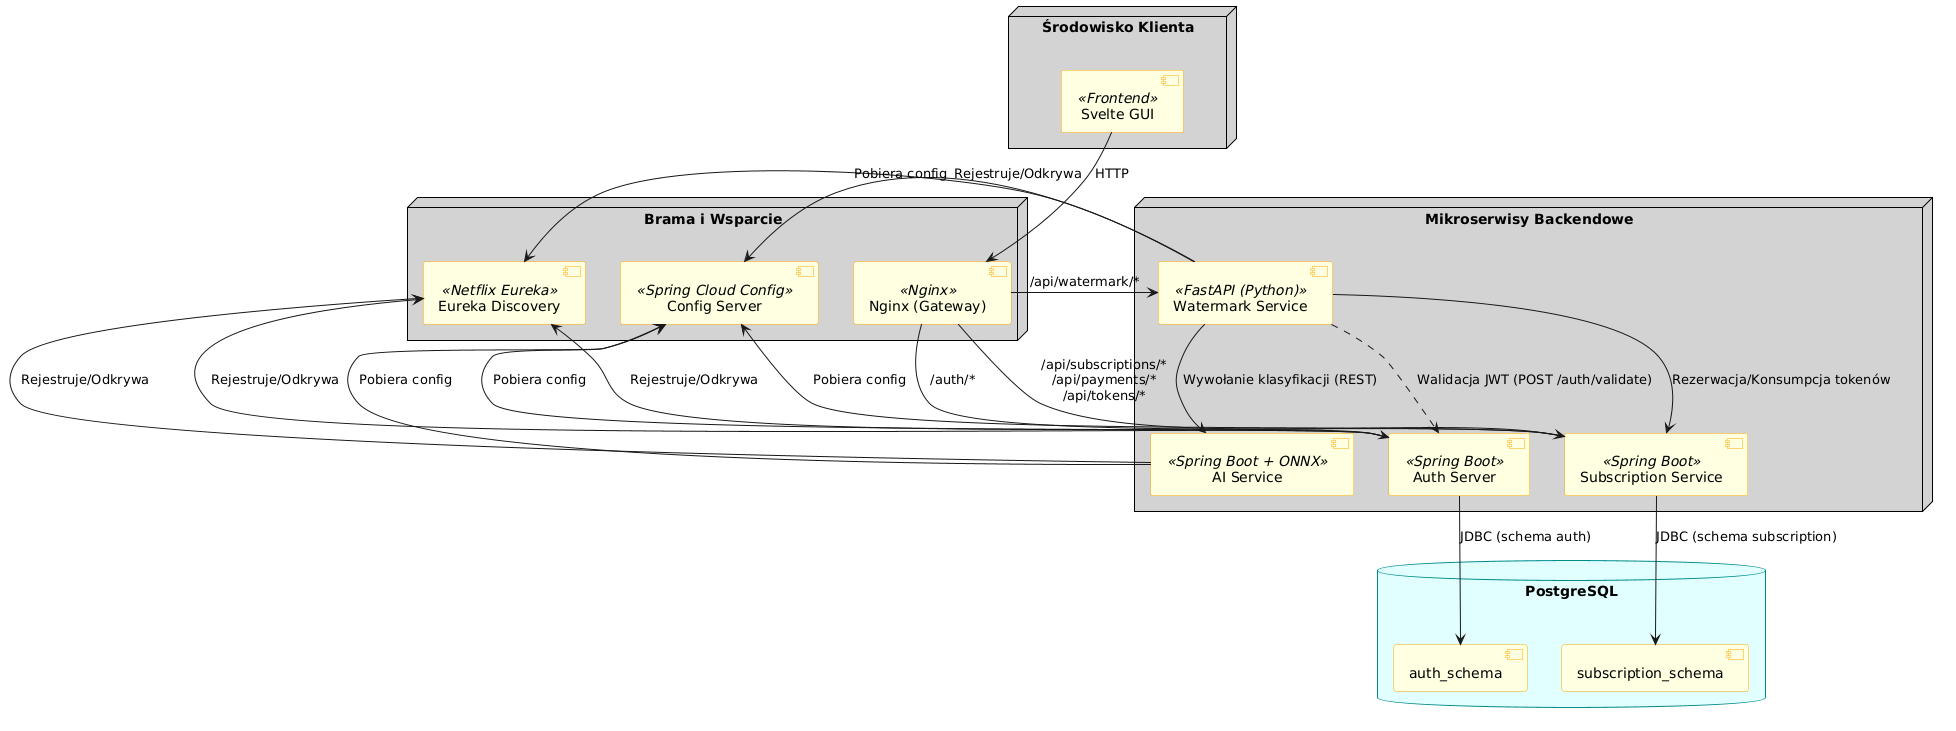
\includegraphics[width=0.95\textwidth]{architecture.png}
    \caption{Architektura mikroserwisowa systemu StegoCloud}
    \label{fig:architecture}
\end{figure}

\subsection{Integracje z zewnętrznymi systemami}
System integruje się z następującymi mechanizmami wspierającymi:
\begin{itemize}
    \item \textbf{Spring Cloud Config Server}: Centralne repozytorium konfiguracyjne przechowujące pliki konfiguracyjne mikroserwisów w dedykowanym repozytorium Git.
    \textit{Zmiany konfiguracji mogą być dynamicznie propagowane.}
    \item \textbf{Spring Cloud Netflix Eureka}: Serwer rejestracji i odkrywania usług (Service Discovery), umożliwiający dynamiczne kierowanie ruchu i skalowalność mikroserwisów.
    \item \textbf{PostgreSQL}: Relacyjna baza danych współdzielona na poziomie instancji, ale logicznie wydzielona na osobne schematy: \texttt{auth\_schema} dla serwera autoryzacji oraz \texttt{subscription\_schema} dla serwisu subskrypcji.
    \item \textbf{ONNX Runtime}: Zintegrowane bibliotecznie w serwisie AI środowisko wykonawcze do uruchamiania wytrenowanego modelu głębokiego uczenia MobileNetV2 bez konieczności instalowania pełnych bibliotek takich jak TensorFlow czy PyTorch.
\end{itemize}

\newpage

% --- 3. DIAGRAMY PRZYPADKÓW UŻYCIA ---
\section{Diagramy przypadków użycia}

\subsection{Diagram ogólny}
Diagram przypadków użycia przedstawia interakcje aktorów (Użytkownik, Administrator oraz zewnętrzna Bramka Płatności) z poszczególnymi funkcjonalnościami systemu StegoCloud.

\begin{figure}[H]
    \centering
    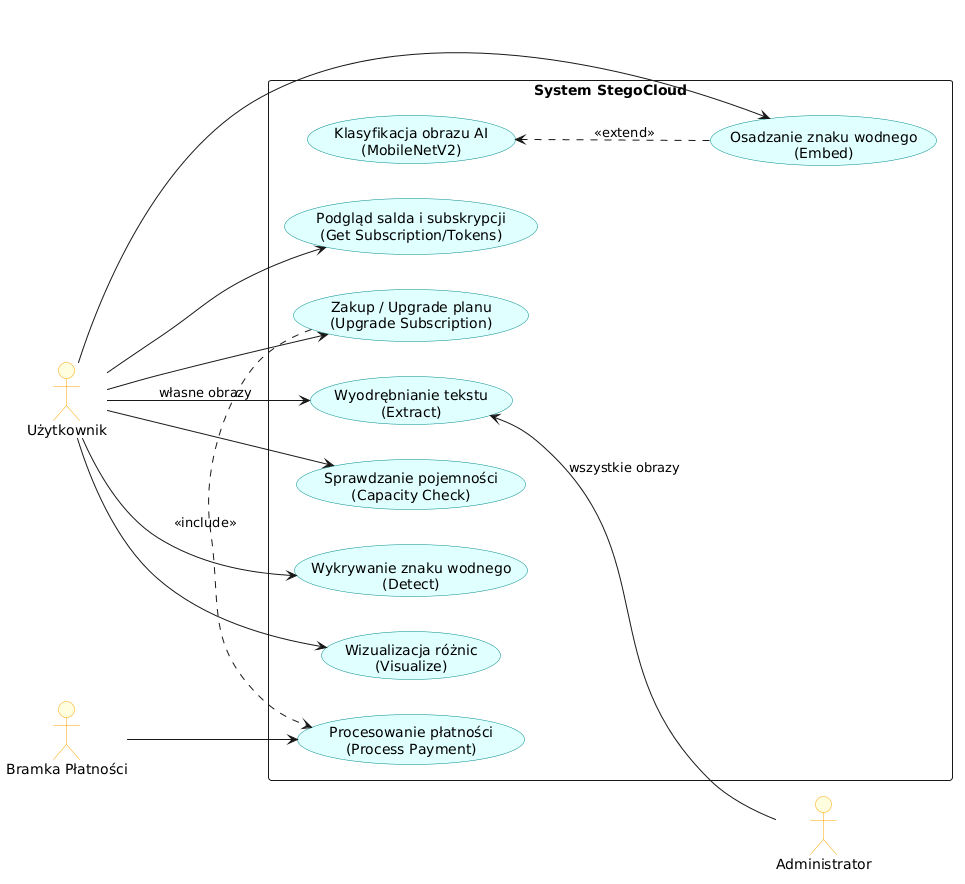
\includegraphics[width=0.85\textwidth]{use_cases.png}
    \caption{Diagram przypadków użycia systemu StegoCloud}
    \label{fig:use_cases}
\end{figure}

\subsection{Opis wybranych przypadków użycia}

Poniższe tabele szczegółowo opisują dwa kluczowe przypadki użycia systemu: osadzanie znaku wodnego z klasyfikacją AI oraz zakup/upgrade planu subskrypcji.

\begin{table}[H]
\centering
\caption{Opis przypadku użycia: Osadzanie znaku wodnego z klasyfikacją AI}
\begin{tabularx}{\textwidth}{lX}
\toprule
\textbf{Nazwa przypadku} & Osadzenie znaku wodnego z klasyfikacją AI \\
\midrule
\textbf{Aktorzy} & Użytkownik Zalogowany, \texttt{watermark-service-py}, \texttt{subscription-service}, \texttt{ai-service} \\
\midrule
\textbf{Warunki wstępne} & 
1. Użytkownik jest zalogowany i posiada ważny token JWT. \newline
2. Użytkownik posiada aktywny plan \texttt{PRO}. \newline
3. Saldo tokenów użytkownika wynosi co najmniej 7 tokenów (koszt embed: 5 lub 8 + koszt AI: 2). \newline
4. Przesłany plik jest poprawnym formatem PNG o wymiarach $\ge 1024 \times 1024$ px. \\
\midrule
\textbf{Przebieg główny} & 
1. Użytkownik wybiera plik PNG oraz wpisuje treść znaku wodnego w GUI. \newline
2. GUI wysyła żądanie do bramki Nginx, która przekazuje je do \texttt{watermark-service-py}. \newline
3. \texttt{watermark-service-py} pyta \texttt{subscription-service} o rezerwację tokenów na operację embedowania. \newline
4. \texttt{subscription-service} dokonuje rezerwacji tokenów o statusie \texttt{RESERVED}. \newline
5. \texttt{watermark-service-py} pyta \texttt{subscription-service} o rezerwację tokenów na klasyfikację AI. Rezerwacja zostaje zatwierdzona. \newline
6. \texttt{watermark-service-py} wysyła obraz do \texttt{ai-service}. \newline
7. \texttt{ai-service} uruchamia model ONNX, klasyfikuje obraz i zwraca etykiety (np. klasyfikacja: "samochód", pewność: 94\%). \newline
8. \texttt{watermark-service-py} przesyła żądanie konsumpcji rezerwacji AI. \newline
9. \texttt{watermark-service-py} szyfruje payload AES-GCM, koduje Reed-Solomon i osadza go w DCT obrazu. \newline
10. Po poprawnym osadzeniu, serwis wysyła żądanie konsumpcji rezerwacji embedowania do \texttt{subscription-service}. \newline
11. Obraz PNG wraz z nagłówkami wyników klasyfikacji AI zostaje przesłany do GUI i udostępniony do pobrania. \\
\midrule
\textbf{Przebieg alternatywny} & 
\textbf{4a/5a. Brak tokenów lub niepoprawny plan}: \texttt{subscription-service} odmawia rezerwacji. Proces zostaje przerwany z błędem 403/409, użytkownik widzi komunikat w GUI. \newline
\textbf{9a. Błąd algorytmu steganograficznego}: \texttt{watermark-service-py} zwalnia rezerwacje tokenów w \texttt{subscription-service} (status \texttt{RELEASED}). Saldo użytkownika nie ulega zmianie. \\
\bottomrule
\end{tabularx}
\end{table}

\newpage

\begin{table}[H]
\centering
\caption{Opis przypadku użycia: Zakup / Upgrade planu subskrypcji}
\begin{tabularx}{\textwidth}{lX}
\toprule
\textbf{Nazwa przypadku} & Zakup / Upgrade planu subskrypcji \\
\midrule
\textbf{Aktorzy} & Użytkownik Zalogowany, \texttt{subscription-service}, Bramka Płatności (Mock) \\
\midrule
\textbf{Warunki wstępne} & 
1. Użytkownik jest zalogowany. \newline
2. Użytkownik posiada aktualnie niższy plan niż docelowy (dozwolone przejścia: \texttt{FREE $\rightarrow$ STANDARD}, \texttt{FREE $\rightarrow$ PRO}, \texttt{STANDARD $\rightarrow$ PRO}). \\
\midrule
\textbf{Przebieg główny} & 
1. Użytkownik w panelu subskrypcji wybiera przycisk "Kup" przy wybranym nowym planie. \newline
2. GUI wysyła żądanie utworzenia sesji płatniczej do \texttt{subscription-service}. \newline
3. \texttt{subscription-service} tworzy sesję płatniczą o statusie \texttt{PENDING} i zwraca jej identyfikator oraz adres bramki płatniczej. \newline
4. GUI przekierowuje użytkownika na stronę bramki płatności (Mock Payment Page). \newline
5. Użytkownik klika przycisk "Zatwierdź płatność". \newline
6. Bramka płatności wysyła żądanie sukcesu płatności do \texttt{subscription-service} przekazując \texttt{sessionId}. \newline
7. \texttt{subscription-service} weryfikuje sesję i jej właściciela, a następnie zmienia status sesji na \texttt{SUCCEEDED}. \newline
8. Serwis modyfikuje subskrypcję użytkownika w bazie (nowy plan, nowa data ważności na +1 miesiąc). \newline
9. Saldo tokenów użytkownika zostaje zasilone pełną pulą nowego planu. \newline
10. Użytkownik zostaje przekierowany z powrotem do aplikacji, gdzie GUI prezentuje zaktualizowany stan konta. \\
\midrule
\textbf{Przebieg alternatywny} & 
\textbf{1a. Downgrade lub zakup tego samego planu}: Backend blokuje operację (błąd 400), informując o niedozwolonym przejściu. \newline
\textbf{5a. Anulowanie płatności}: Użytkownik klika "Anuluj". Bramka wysyła status anulowania. Status sesji w bazie zmienia się na \texttt{CANCELLED}. Subskrypcja użytkownika pozostaje bez zmian. \\
\bottomrule
\end{tabularx}
\end{table}

\newpage

% --- 4. DIAGRAM KOMPONENTÓW ---
\section{Diagram komponentów}

\subsection{Diagram komponentów}
Diagram komponentów przedstawia dekompozycję systemu na poszczególne moduły aplikacyjne, interfejsy komunikacyjne oraz zależności między nimi.

\begin{figure}[H]
    \centering
    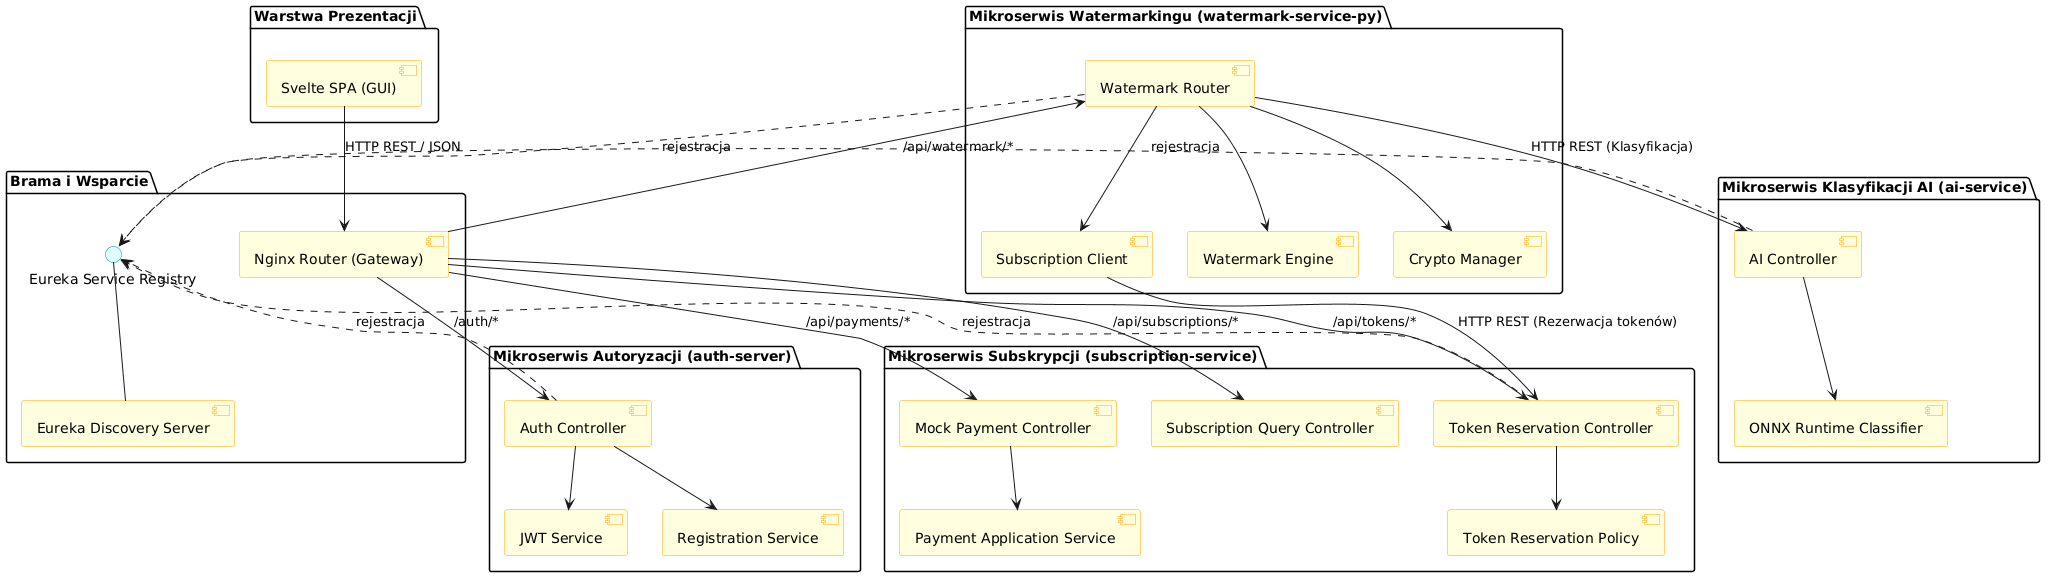
\includegraphics[width=0.95\textwidth]{components.png}
    \caption{Diagram komponentów systemu StegoCloud}
    \label{fig:components}
\end{figure}

\subsection{Opis komponentów}
\begin{itemize}
    \item \textbf{Svelte SPA (GUI)}: Aplikacja kliencka uruchamiana w przeglądarce użytkownika. Odpowiada za prezentowanie formularzy, obsługę plików PNG, podgląd heatmap i zarządzanie profilami subskrypcji.
    \item \textbf{Nginx Router (Gateway)}: Odpowiada za kierowanie ruchu zewnętrznego (routing) do odpowiednich mikroserwisów na podstawie prefiksów ścieżek URL, pełniąc funkcję API Gateway.
    \item \textbf{Auth Controller \& JWT Service}: Części składowe \texttt{auth-server}. Odpowiadają za weryfikację haseł (BCrypt), generowanie tokenów JWT oraz rejestrację nowych użytkowników.
    \item \textbf{Token Reservation \& Subscription Controller}: Komponenty \texttt{subscription-service}. Odpowiadają odpowiednio za przyjmowanie żądań rezerwacji tokenów oraz zarządzanie sesjami płatniczymi i planami.
    \item \textbf{Watermark Router \& Engine}: Komponenty usługi \texttt{watermark-service-py}. Router wystawia punkty końcowe (REST API), a Engine wykonuje algorytm częstotliwościowy przy użyciu biblioteki \texttt{invisible-watermark}.
    \item \textbf{Crypto Manager}: Komponent pomocniczy usługi watermarkingu. Szyfruje tekst znaku wodnego z użyciem AES-GCM przed osadzeniem, używając klucza wyprowadzonego z sekretu aplikacji.
    \item \textbf{AI Controller \& ONNX Runtime Classifier}: Części składowe \texttt{ai-service}. Pobierają obraz i przekazują go do silnika ONNX Runtime uruchamiającego sieć MobileNetV2, która wykonuje klasyfikację.
\end{itemize}

\newpage

% --- 5. DIAGRAM KLAS ---
\section{Diagram klas}

\subsection{Diagram klas}
Diagram klas prezentuje kluczowe encje bazodanowe, rekordy oraz interfejsy wchodzące w skład warstwy domenowej systemów \texttt{subscription-service}, \texttt{auth-server} oraz strukturę modułu w \texttt{watermark-service-py}.

\begin{figure}[H]
    \centering
    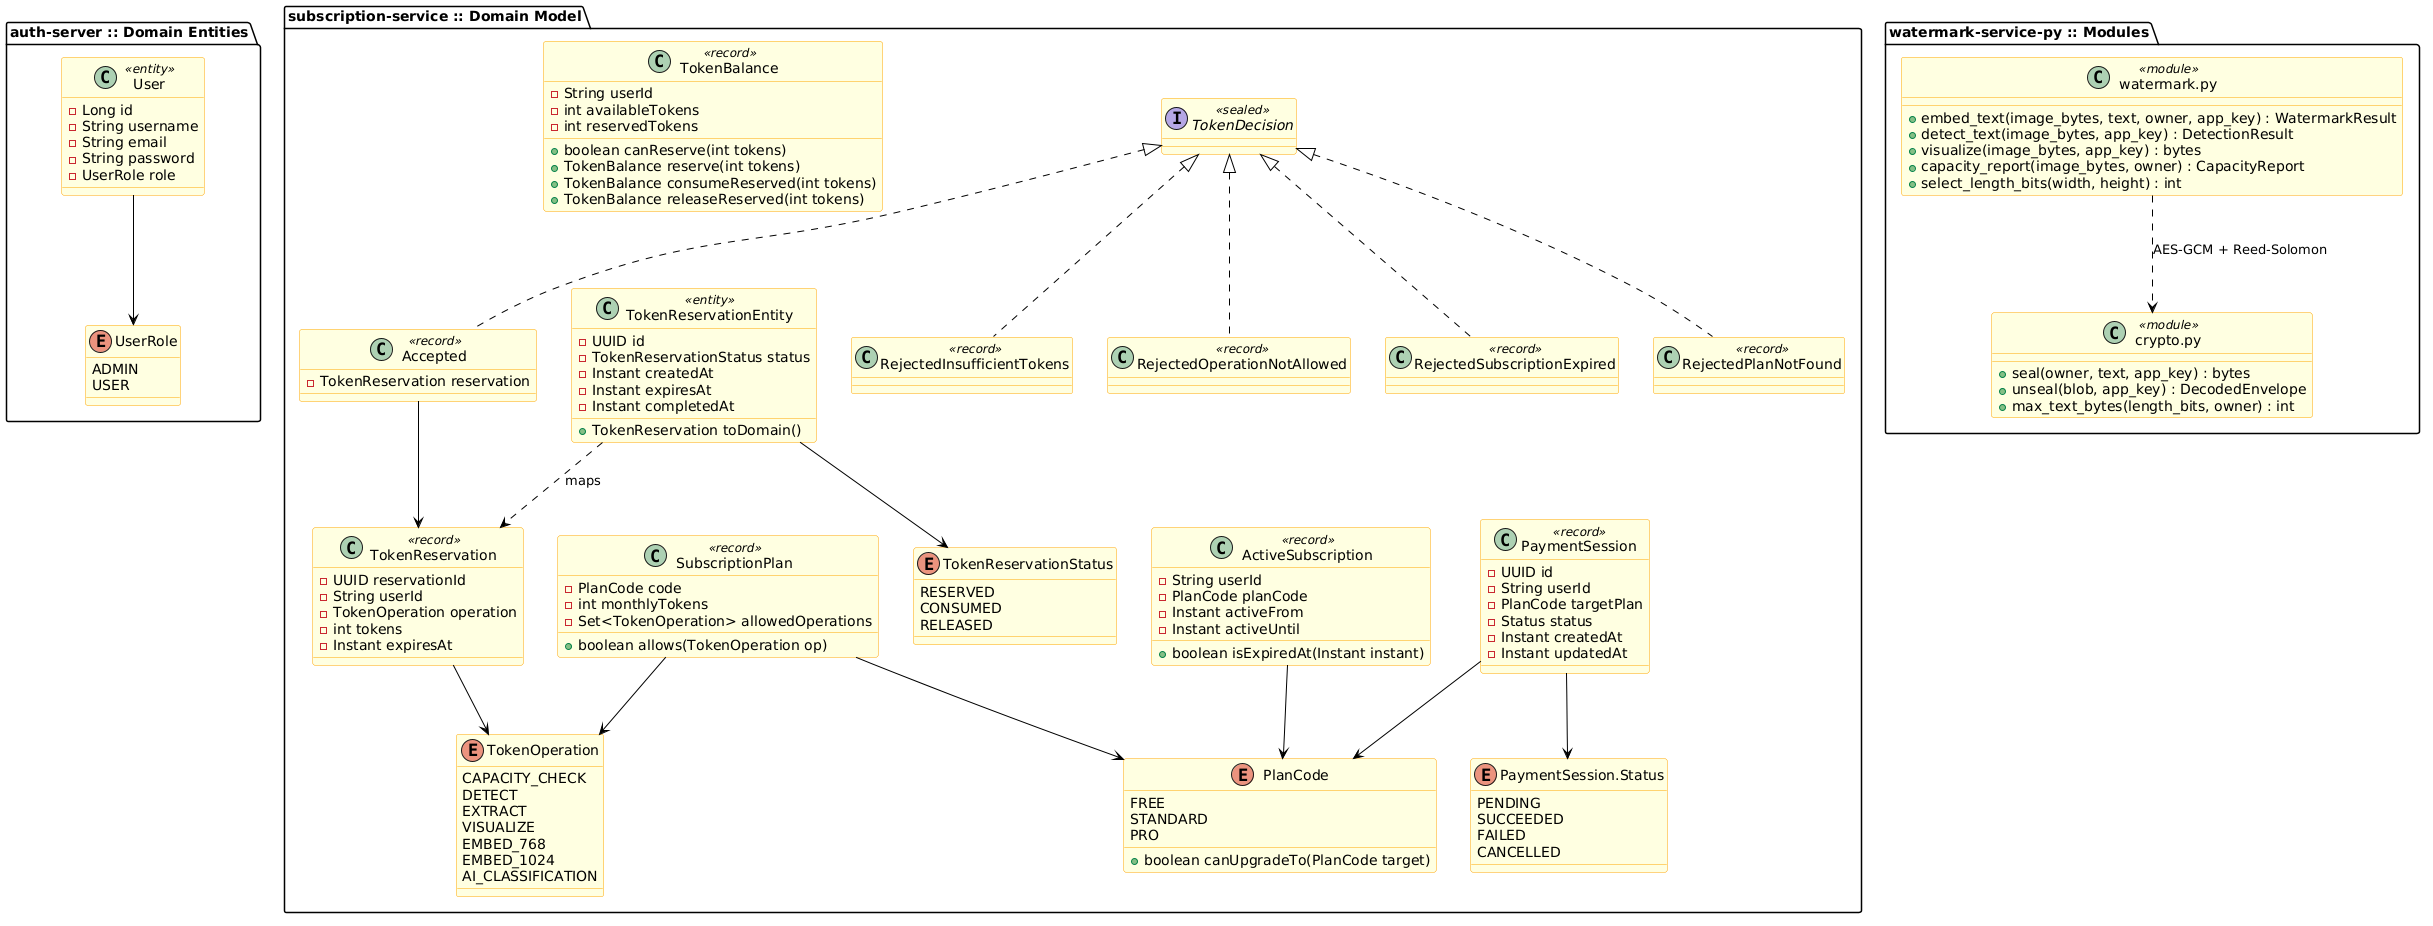
\includegraphics[width=0.98\textwidth]{classes.png}
    \caption{Diagram klas domenowych systemu StegoCloud}
    \label{fig:classes}
\end{figure}

\subsection{Opis kluczowych struktur danych}
\begin{itemize}
    \item \textbf{User \& UserRole}: Reprezentują użytkownika w systemie autoryzacji wraz z rolą przypisaną na potrzeby kontroli dostępu na poziomie endpointów (RBAC).
    \item \textbf{SubscriptionPlan}: Klasa definiująca właściwości planu taryfowego -- liczbę darmowych tokenów na miesiąc oraz zbiór dozwolonych operacji (\texttt{allowedOperations}).
    \item \textbf{ActiveSubscription}: Rekord domenowy reprezentujący powiązanie użytkownika z konkretnym planem (\texttt{planCode}) wraz z okresem jego ważności (\texttt{activeFrom}, \texttt{activeUntil}). Posiada metodę \texttt{isExpiredAt(Instant)} określającą ważność subskrypcji.
    \item \textbf{TokenBalance}: Rekord reprezentujący bilans tokenów zalogowanego użytkownika. Zawiera informację o tokenach dostępnych (\texttt{availableTokens}) oraz zablokowanych na poczet trwających operacji (\texttt{reservedTokens}).
    \item \textbf{TokenReservation}: Reprezentuje rezerwację tokenów dokonaną przez system podczas rozpoczęcia operacji steganograficznej. Rekord domenowy zawiera unikalne ID (\texttt{UUID}), typ operacji oraz koszt tokenowy, natomiast status cyklu życia (\texttt{RESERVED}, \texttt{CONSUMED}, \texttt{RELEASED}) jest utrwalany w encji \texttt{TokenReservationEntity}.
    \item \textbf{TokenDecision}: Zamknięty interfejs (\texttt{sealed interface}), który przy użyciu mechanizmów Javy 21 wymusza kompletną obsługę wszystkich możliwych decyzji biznesowych dotyczących przydziału tokenów (akceptacja lub konkretny powód odmowy).
\end{itemize}

\newpage

% --- 6. DIAGRAMY INTERAKCJI ---
\section{Diagramy interakcji}

\subsection{Diagram interakcji: Osadzenie znaku wodnego z klasyfikacją AI}
Diagram przedstawia sekwencję komunikatów i wywołań API podczas osadzania tekstu w obrazie z opcjonalną weryfikacją zawartości przez sztuczną inteligencję.

\begin{figure}[H]
    \centering
    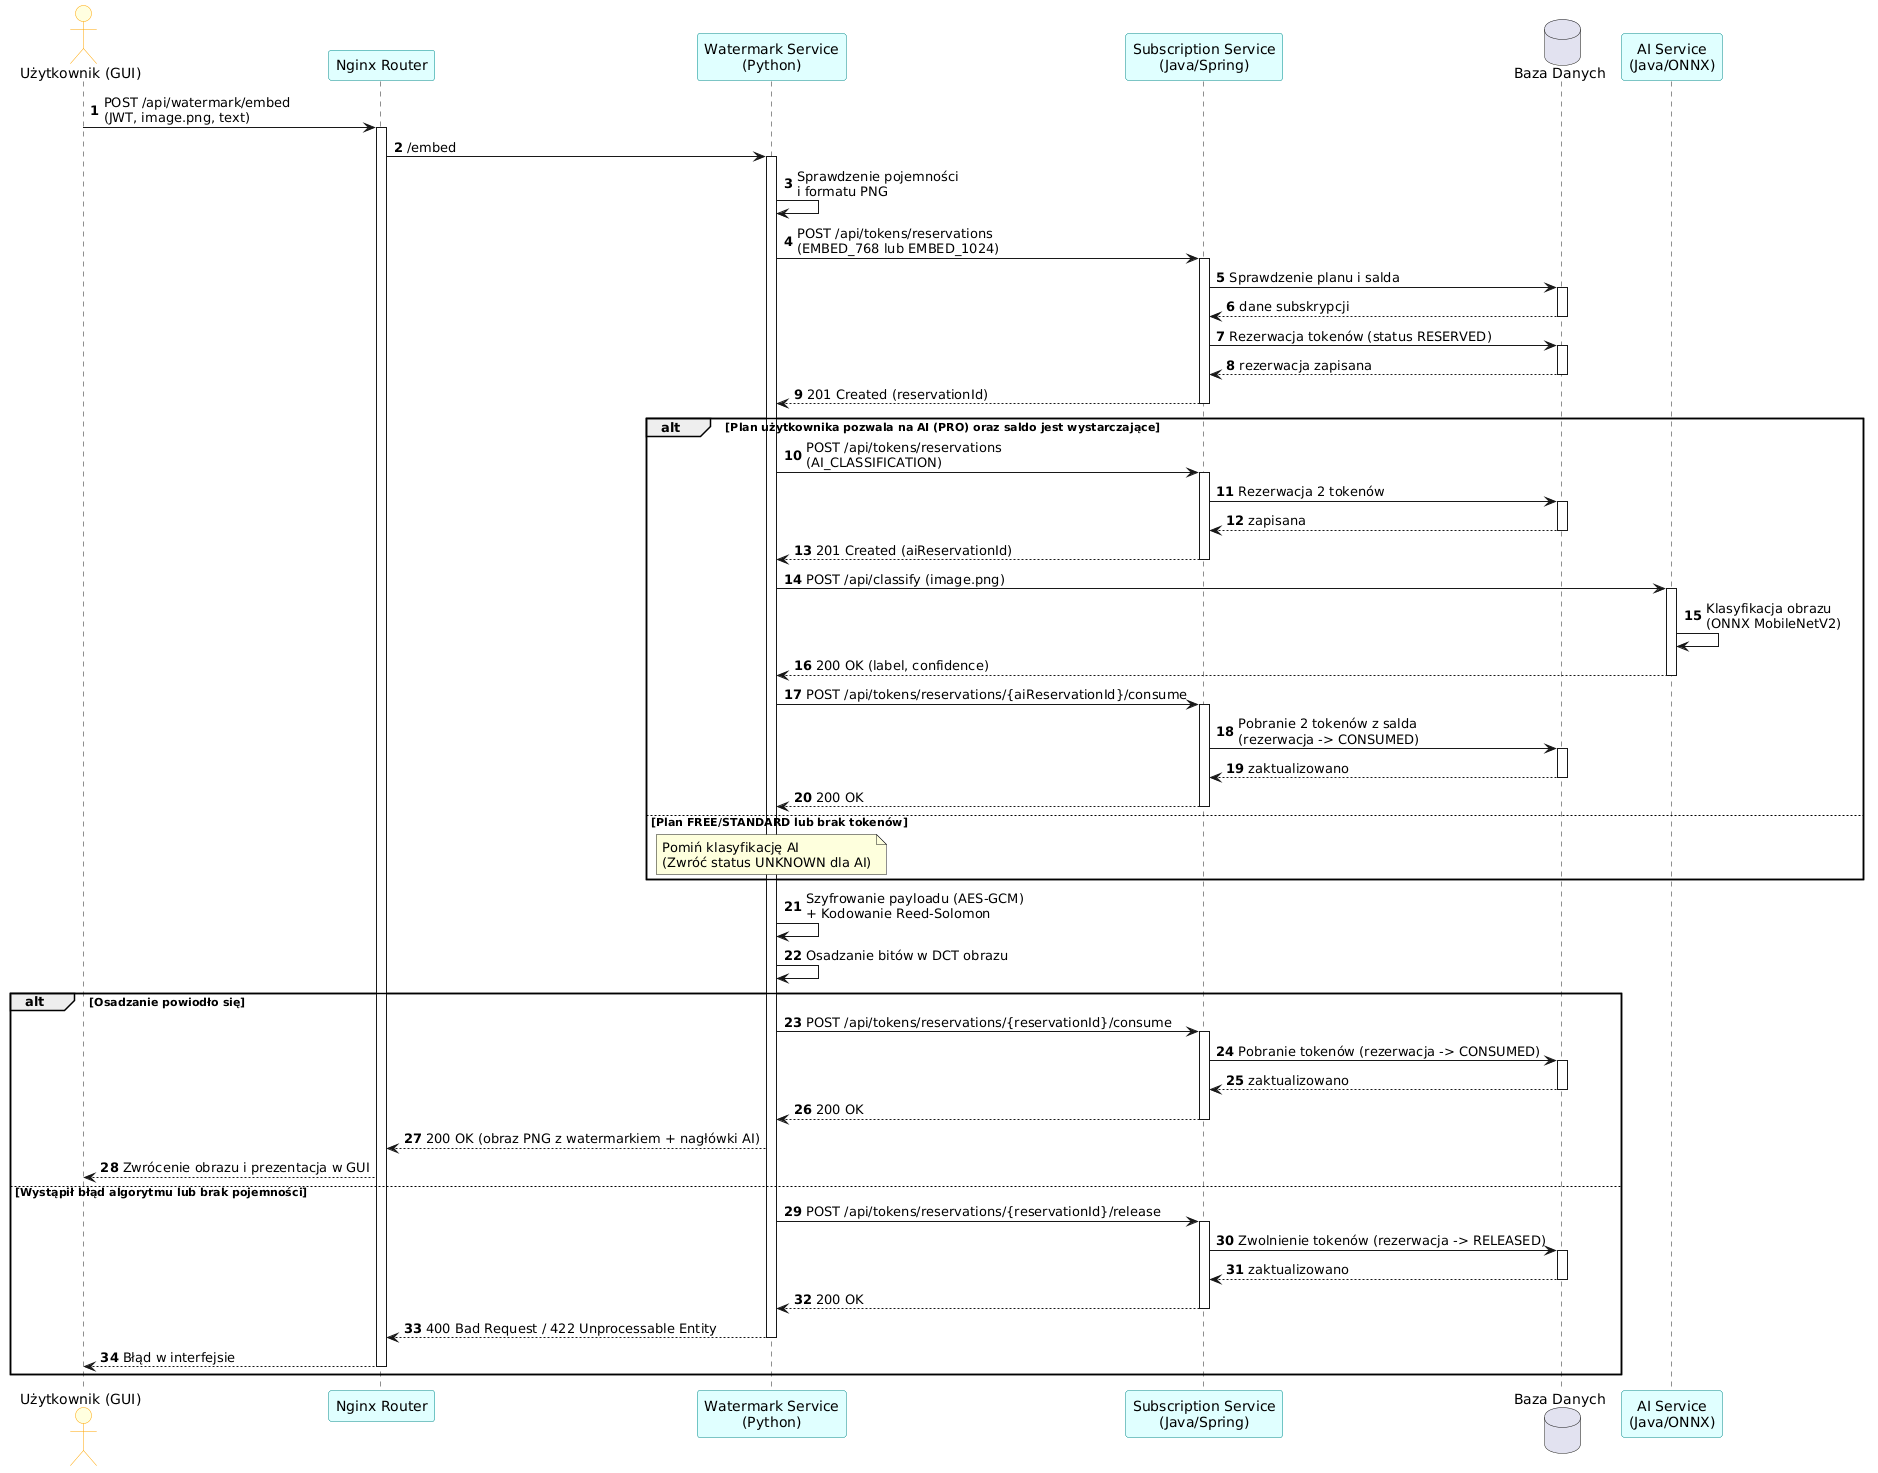
\includegraphics[width=0.98\textwidth]{seq_embed_ai.png}
    \caption{Diagram sekwencyjny: Proces osadzania znaku wodnego z klasyfikacją AI}
    \label{fig:seq_embed_ai}
\end{figure}

\subsection{Diagram interakcji: Zakup / Upgrade planu subskrypcji}
Diagram przedstawia przebieg rejestracji sesji płatniczej, jej opłacenia oraz ostatecznej aktualizacji danych abonamentowych w bazie danych.

\begin{figure}[H]
    \centering
    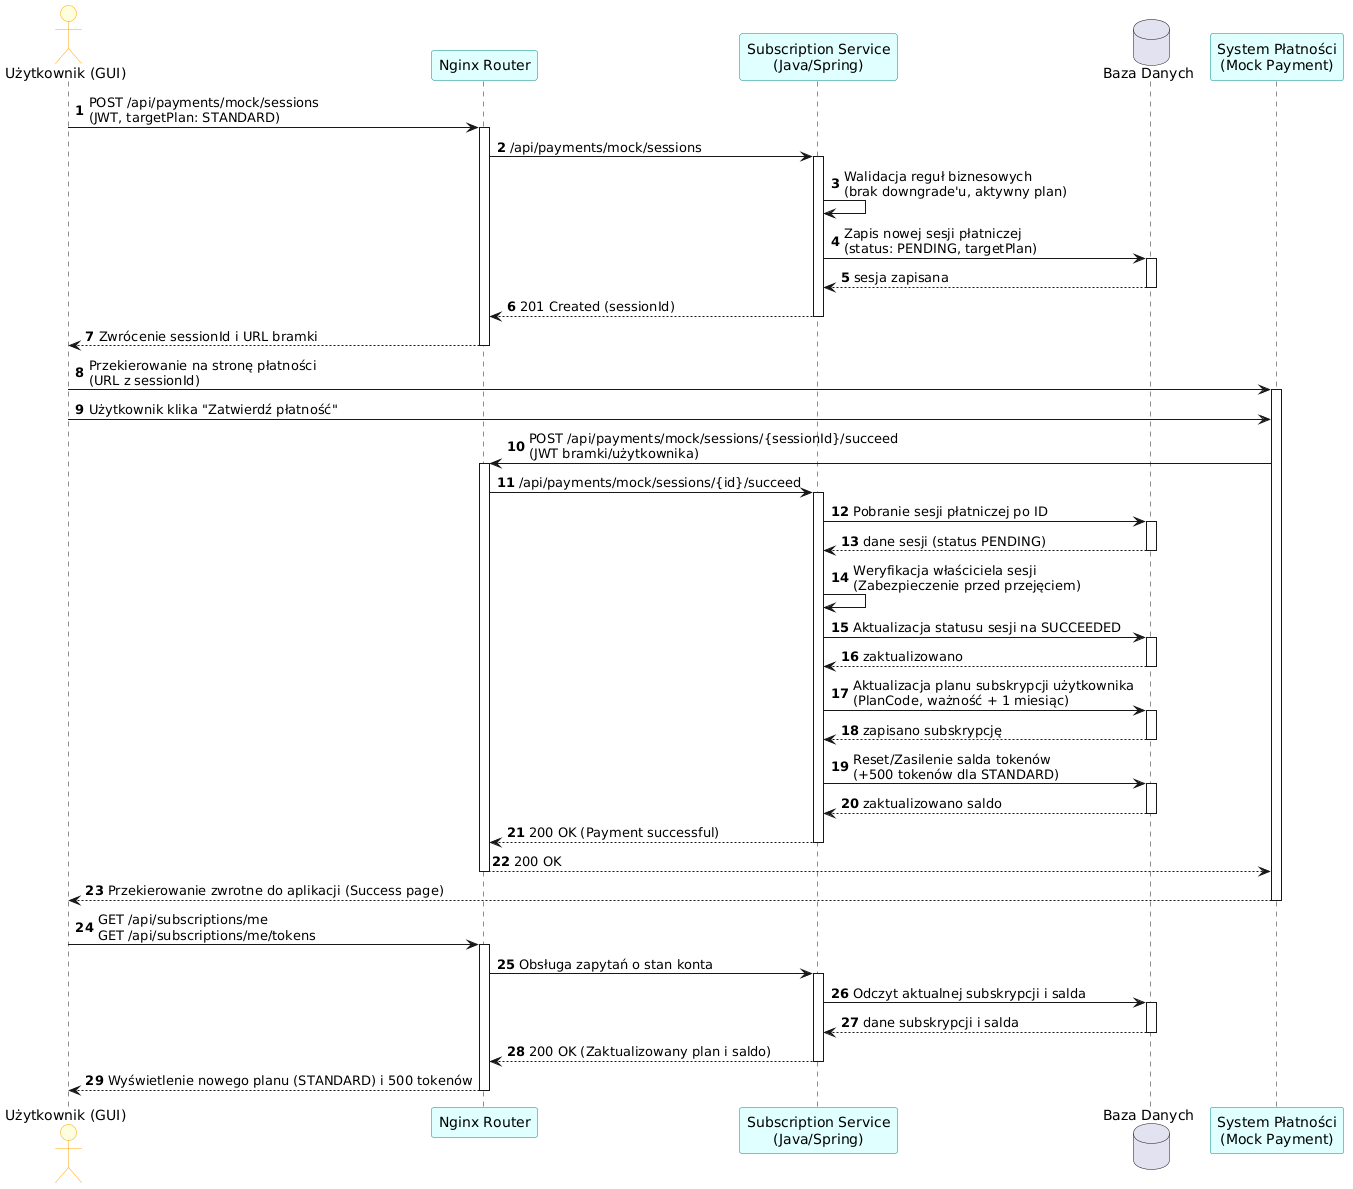
\includegraphics[width=0.98\textwidth]{seq_subscription_upgrade.png}
    \caption{Diagram sekwencyjny: Proces zakupu / upgrade'u planu subskrypcji}
    \label{fig:seq_sub_upgrade}
\end{figure}

\newpage

% --- 7. STACK TECHNOLOGICZNY ---
\section{Stack technologiczny}

Wybrane komponenty systemu zostały zaimplementowane przy użyciu technologii dobranych pod kątem ich zalet wydajnościowych oraz spełnienia celów dydaktycznych i biznesowych projektu.

\begin{table}[H]
\centering
\caption{Wykorzystane technologie i uzasadnienie wyboru}
\begin{tabularx}{\textwidth}{l|p{4cm}|X}
\toprule
\textbf{Komponent} & \textbf{Technologia} & \textbf{Uzasadnienie wyboru} \\
\midrule
Backend Core & Java 21 / Spring Boot 3 & Zapewnia stabilne środowisko, wysokie bezpieczeństwo typów oraz wsparcie dla najnowszych funkcjonalności JDK (rekordy, dopasowywanie wzorców dla switcha, sealed classes), które upraszczają kod domeny subskrypcji. \\
\midrule
Steganografia & Python 3.12 / FastAPI & Znakowanie obrazów wymaga niskopoziomowych operacji matematycznych (DWT-DCT-SVD) oraz wsparcia dla zaawansowanych bibliotek naukowych (NumPy, OpenCV, invisible-watermark). FastAPI zapewnia asynchroniczność oraz generuje automatyczną dokumentację OpenAPI. \\
\midrule
AI/Klasyfikacja & ONNX Runtime (Java) & Umożliwia ładowanie i szybkie uruchamianie modeli sieci neuronowych (\texttt{MobileNetV2} wyeksportowanego z PyTorch) bezpośrednio w procesie Javy z optymalizacją sprzętową, bez potrzeby stawiania ciężkiego środowiska PyTorch. \\
\midrule
Baza Danych & PostgreSQL 17 & Stabilna, relacyjna baza danych obsługująca transakcje ACID niezbędne w logice rozliczania tokenów i płatności. Zapewnia izolację za pomocą osobnych schematów bazodanowych. \\
\midrule
Frontend GUI & Svelte 5 (SvelteKit) / nginx & Svelte generuje niezwykle lekki kod kliencki (brak narzutu Virtual DOM), co przekłada się na szybkie ładowanie interfejsu. Nginx służy jako serwer statyczny i Gateway proxy. \\
\midrule
Narzędzia & Docker Compose / SonarQube & Konteneryzacja ułatwia lokalne uruchamianie całego rozproszonego środowiska. SonarQube umożliwia ciągłą analizę statyczną kodu w celu utrzymania długu technicznego na niskim poziomie. \\
\bottomrule
\end{tabularx}
\end{table}

\newpage

% --- 8. DZIAŁANIE SYSTEMU ---
\section{Działanie systemu}

W tej sekcji przedstawiono kluczowe zrzuty ekranu prezentujące działanie systemu StegoCloud, wykonane na uruchomionej instancji (użytkownik \texttt{pro} z planem \texttt{PRO}).

\subsection{Zrzuty ekranu interfejsu użytkownika}

\begin{figure}[H]
    \centering
    \begin{subfigure}[t]{0.45\textwidth}
        \centering
        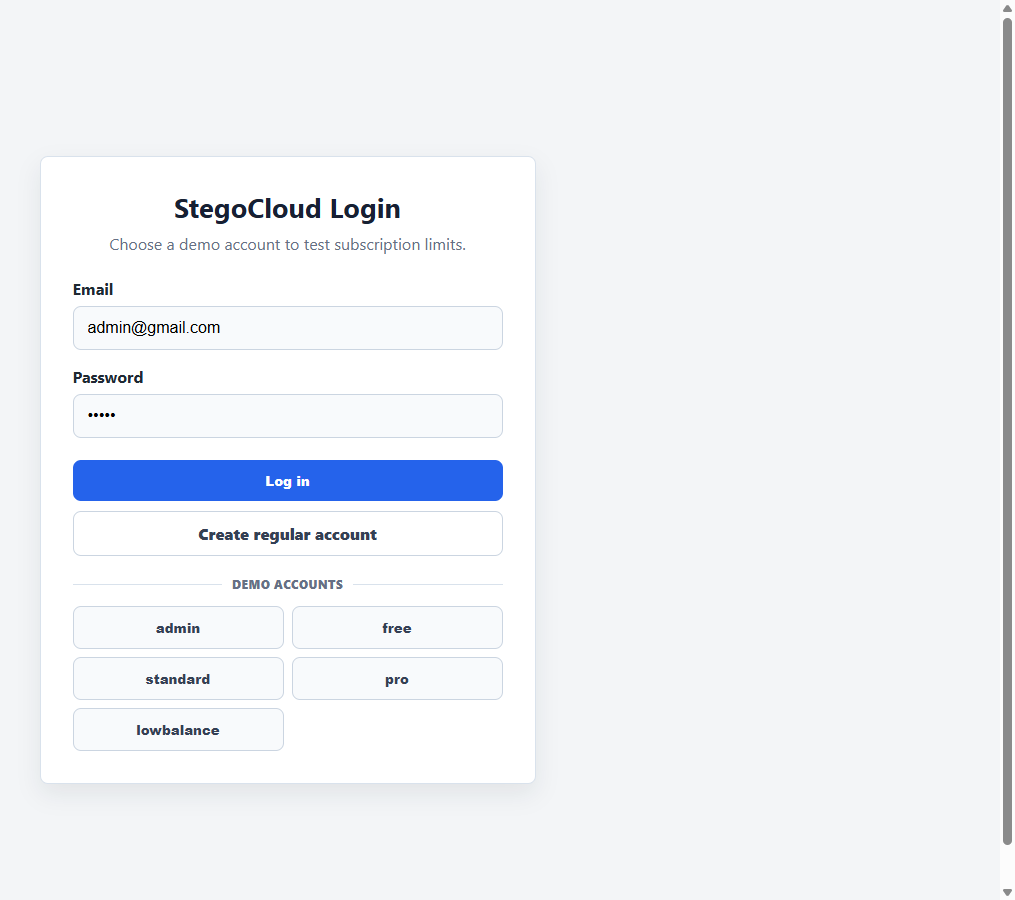
\includegraphics[width=\textwidth]{screen_login.png}
        \caption{Ekran logowania z kontami demonstracyjnymi}
    \end{subfigure}
    \hfill
    \begin{subfigure}[t]{0.53\textwidth}
        \centering
        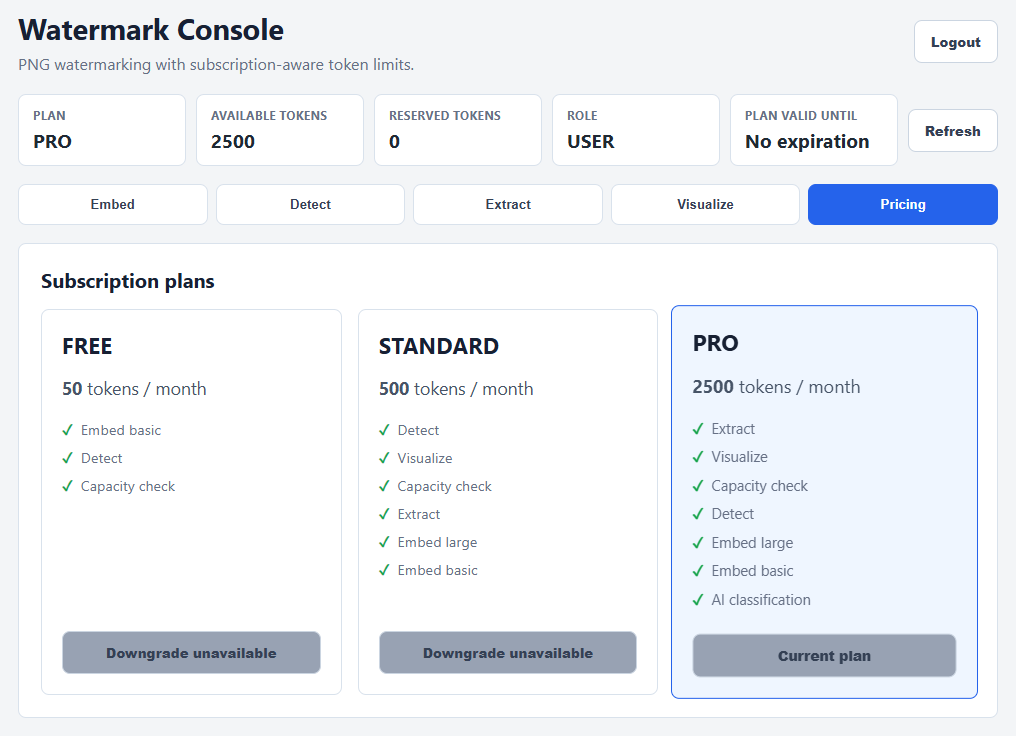
\includegraphics[width=\textwidth]{screen_subscription.png}
        \caption{Panel planów subskrypcji wraz z saldem tokenów}
    \end{subfigure}
    \caption{Ekran logowania oraz panel wyboru planu subskrypcji (Free, Standard, Pro) i salda tokenów}
    \label{fig:screen_login}
\end{figure}

\begin{figure}[H]
    \centering
    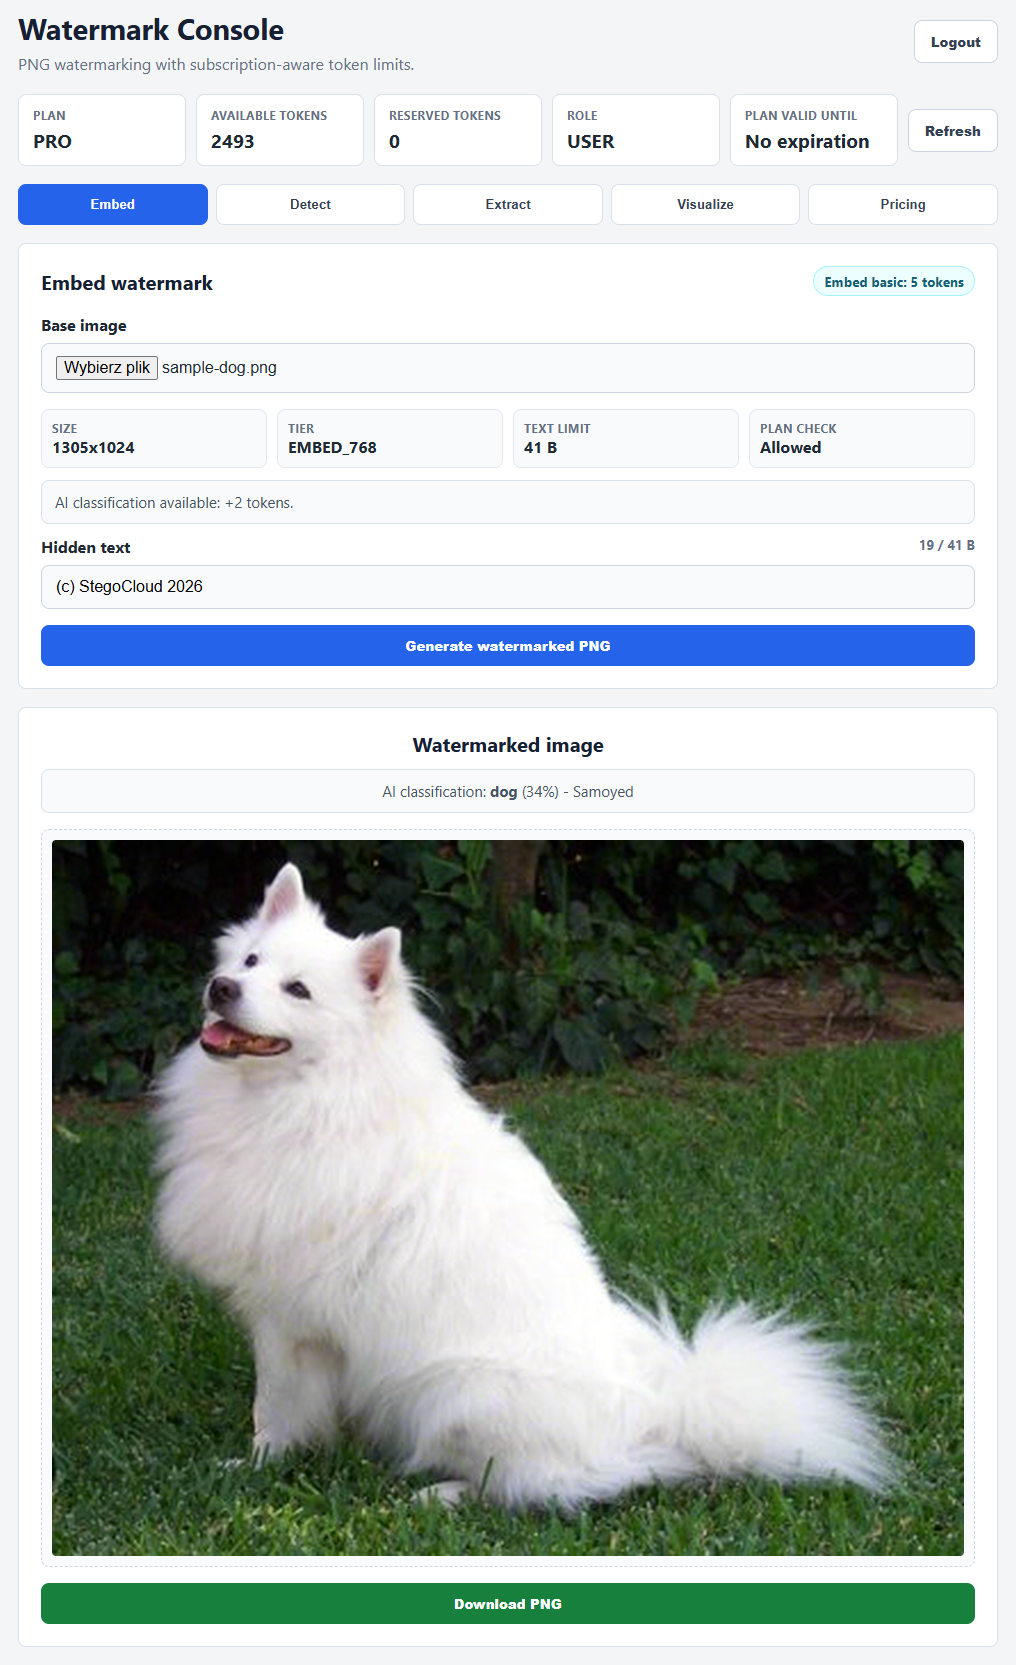
\includegraphics[width=0.56\textwidth]{screen_embed.png}
    \caption{Panel osadzania znaku wodnego: Capacity Check (rozmiar, tier \texttt{EMBED\_768}, limit tekstu, kontrola planu), klasyfikacja AI (\texttt{dog}, ufność 34\%) oraz wynikowy obraz PNG ze znakiem wodnym}
    \label{fig:screen_embed}
\end{figure}

\begin{figure}[H]
    \centering
    \begin{subfigure}[t]{0.49\textwidth}
        \centering
        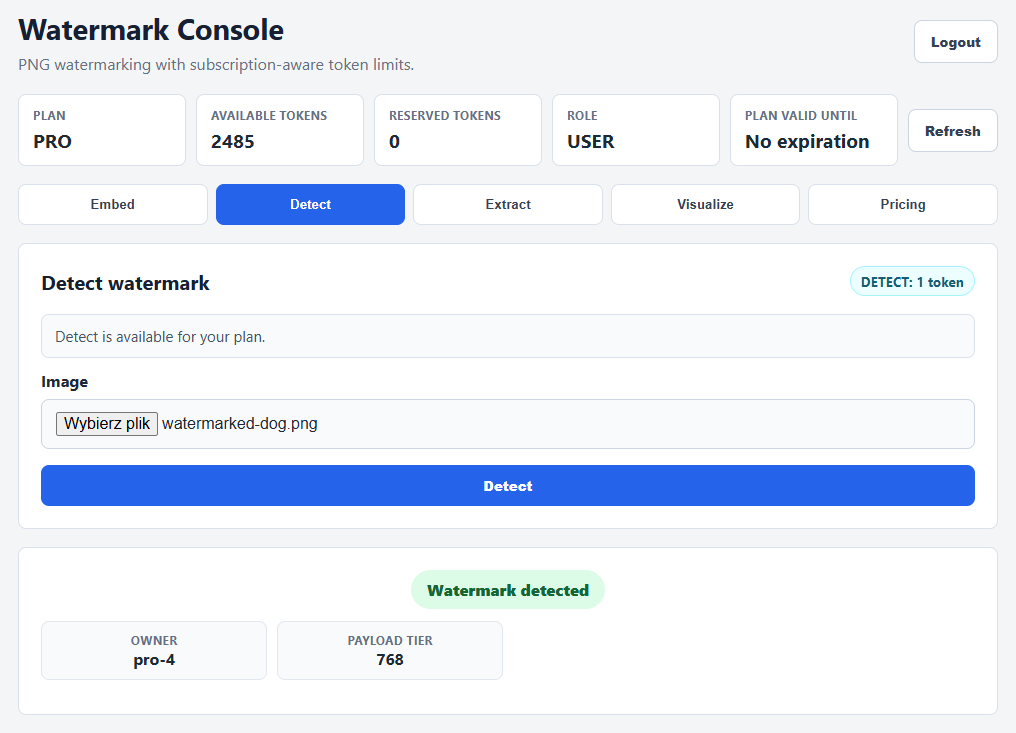
\includegraphics[width=\textwidth]{screen_detect.png}
        \caption{Detekcja: wykryty znak wodny i tożsamość właściciela (\texttt{pro-4})}
    \end{subfigure}
    \hfill
    \begin{subfigure}[t]{0.49\textwidth}
        \centering
        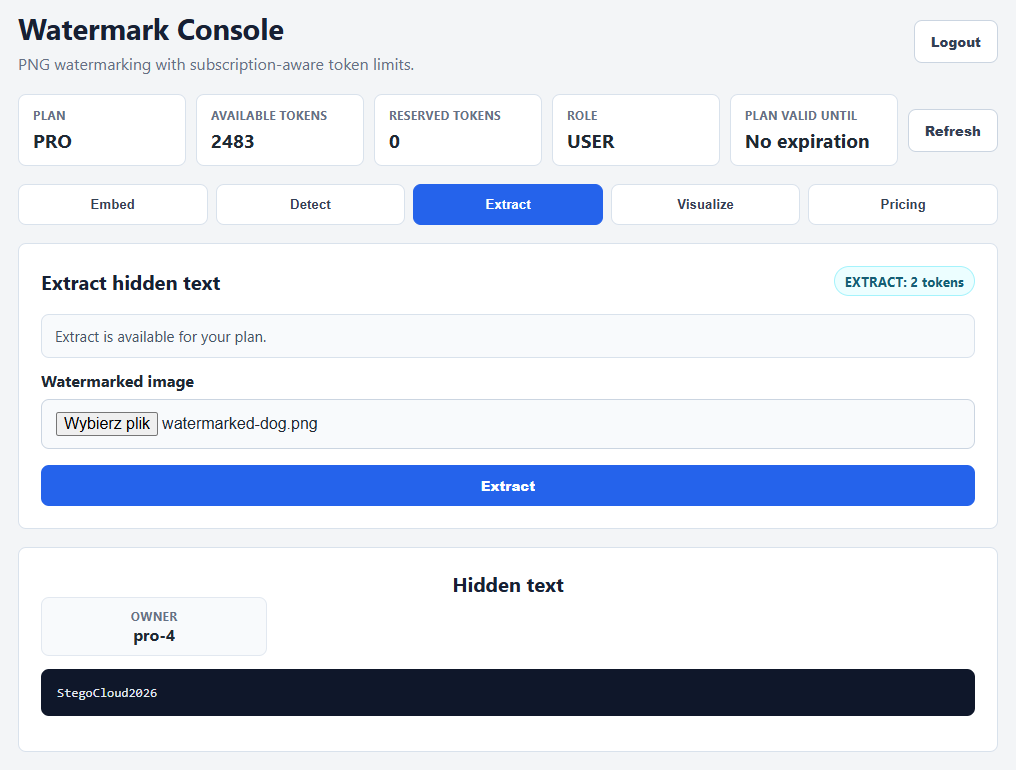
\includegraphics[width=\textwidth]{screen_extract.png}
        \caption{Ekstrakcja: odczytany ukryty tekst (\texttt{StegoCloud2026})}
    \end{subfigure}

    \vspace{0.4cm}
    \begin{subfigure}[t]{0.5\textwidth}
        \centering
        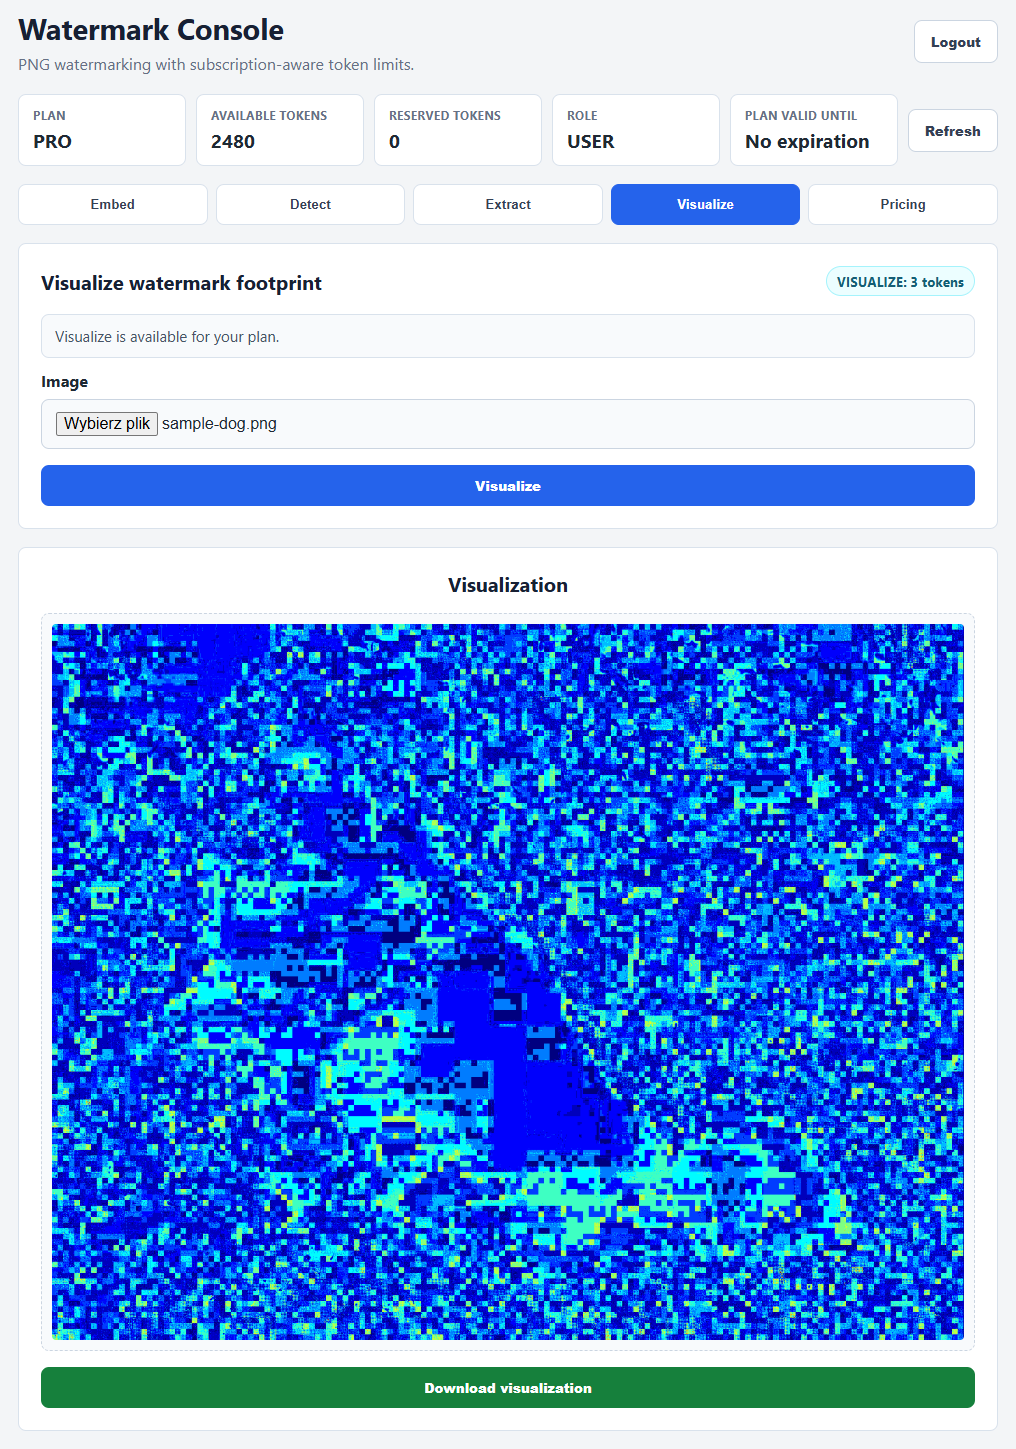
\includegraphics[width=\textwidth]{screen_visualize.png}
        \caption{Wizualizacja: heatmapa różnic pikseli (pixel-diff)}
    \end{subfigure}
    \caption{Detekcja znaku wodnego, ekstrakcja ukrytego tekstu oraz wizualizacja heatmapy różnic}
    \label{fig:screen_detect}
\end{figure}

\newpage

% --- 9. PODSUMOWANIE ---
\section{Podsumowanie}
Projekt \textbf{StegoCloud} z powodzeniem integruje zaawansowane mechanizmy platformy Java 21, architekturę mikroserwisową Spring Cloud oraz dedykowany silnik przetwarzania obrazów w języku Python. 

Dzięki zastosowaniu wzorca rezerwacji tokenów system gwarantuje odporność na błędy sieciowe i transakcyjne -- użytkownicy są obciążani tokenami wyłącznie za operacje, które zostały pomyślnie zakończone. Zastosowanie szyfrowania kopertowego AES-GCM oraz Reed-Solomon ECC w warstwie steganografii gwarantuje wysoki poziom poufności i odporności na zakłócenia. System spełnia wymagania stawiane nowoczesnym aplikacjom korporacyjnym, a jego modularna budowa pozwala na łatwe dodawanie kolejnych algorytmów znakowania oraz modeli klasyfikacji AI w przyszłości.

\end{document}
